\chapter{Organisations are living beings}
\addcontentsline{toc}{chapterdescription}{Organisations, and especially for-profit businesses, are an essential and natural part of human society; so they are best understood as living beings, living systems that have meaning\hyp{}making capacity. To lead our businesses well we need to know their organisational energy economy (and our personal one). Two useful lenses to use are the four integral quadrants, yielding the management accountability hierarchy vs. the human capability hierarchy; and the four layers: intra-personal, inter-personal, intra-organisation, inter-organisation and stakeholders. The problem of purpose, and how to solve it through driver orientation. }
\label{chapter:who-is-your-organisation-base}


\begin{chapterquotation}
Organisations exist to make every individual's strengths productive and their weaknesses irrelevant.\\
\raggedleft\textemdash Peter Drucker\index{Drucker, Peter}
\end{chapterquotation}






\section{Why we need business}
Three central elements of modern life: capitalism, scientific research, and manufacturing, are at the centre of the huge increase in humans thriving. They succeeded in turning the scarcities in financial capital, intellectual capital, manufactured capital, and food into the abundance many of us enjoy today. I (Graham) remember my Granny saying that the modern invention that had improved her life the most was the indoor bathroom, with hot and cold running water.


Business, as currently designed, has done phenomenally well. There is more than enough money, food and housing for every single person in the world to live a better life than the nobility could four centuries ago, and way better than anyone could 4,000 plus years ago. 


However, business as it’s currently designed is no longer fit for purpose. It’s clear that we are  facing two new, interwoven drivers that, unless used to trigger a fundamental reinvention of business, will continue to grow as threats to each of us today and in the future. 


\begin{enumerate}
\item The first driver is the abundance that modern business has created is growing less and less evenly distributed. Global inequality\index{inequality} between rich and poor continues to grow. The fact that in 2020 a disabled man starved to death in Britain because changes to the disability support system left him unable to afford food is a smoking gun signal. We need a way of distributing our global abundance more evenly, i.e., an economy that provisions all. 


\item The second driver is the environmental and social capitals, the foundational capitals for all life, including yours, are being severely overspent. We are eating into our capitals\index{capitals} so fast that we are close to the point of irreversible civilisation collapse. We need a fast way of regenerating, i.e., growing, all these capitals. 
\end{enumerate}


Failing to act on these drivers means the end of this cycle of human civilisation, just as  previous civilisations have been ended by the same drivers\cite{diamond-collapse}. The Roman civilisation ended because they needed more environmental resources than their environmental capital base could provide, like the children of a wealthy family spending all the money accumulated by their parents, rather than spending only the sustainable income generated by working the capital.


How did we get into this mess? 


Perhaps the first multinational recognisably similar to the multinational of today was the Dutch East India company\index{Dutch East India}. This company was incorporated by charter of the Queen, to address the biggest scarcity of that time: financial capital. Up to then, anyone engaged in business had to either provide the capital needed to start the business themselves, or obtain it from their friends and family.


The driver for creating the incorporated organisation was the growing demand in Europe for spices, tea and other limited commodities from distant lands. The cost of building the multinational business necessary to transport these valuable commodities from Asia required more financial capital than any single family could gather through their relationships with their trusted friends. 


Given that driver, an incorporated business capable of attracting risk capital from strangers was the answer.


The limited company as we know it today has been perfected to solve the adaptive challenge of creating trust between people who do not know each other. Sufficient trust for them to risk some or even all of their wealth in the enterprise of complete strangers. 


If a stranger walked up to you in the street and asked you to give them 50\% of your total wealth, to be locked down for the next 20 years in a risky endeavour, what would you answer? The collective answer society has built up over the past four centuries is the modern private and public limited company.


The problem we have today lies in just how well business was designed as a tool to do the job of attracting financial capital. To do that, it was designed to maximally multiply financial capital, without any balance across the other capitals.\index{capitals} 


Of course, in our new design, we need to keep all the good things that business and capitalism brings us, as we redesign it to eliminate all the harm. This means expanding the design of business to one that multiplies, i.e., regenerates, all capitals.






\section{Why we need organisations}
To do together what cannot be done alone. To rise to challenges bigger than the strength of one person, and to attract, multiply, and distribute the scarcest valuable resources. Or, as Gabriel Grant puts it\cite{grant-determination}, we need organisations to maximise our individual and joint capacity for self-determination; i.e., fully human organisations, the  \emph{Humanocracy}\cite{hamel-humanocracy} of Gary Hamel and Michele Zanini.


Human organisations are as old as the first hunter who went out with a friend and set up a deliberate ambush to bring an antelope home for dinner. 


If you think of what human beings are good at, none of our physical strengths are anywhere near the best in class in the rest of the animal kingdom. None of us come anywhere near the long-distance endurance of a migratory bird, nor the top end speed of a cheetah, nor the sheer strength of an elephant, or the power-to-weight ratio of a flea.


What we excel at is organising ourselves into teams, and our tasks into sequence, because we are best in class at picking up on other people's emotions, and bonding together into communities or working teams by using stories to build common ground and common purpose. Organisations\index{organisation} have existed since time immemorial. Whenever we have faced a challenge beyond the strengths of any individual human being, we have organised until our collective strengths have been big enough to overcome the challenge. 


Strong as the woolly mammoth was, it was no match for a large group of humans working together in an organised way. Stories bonded everyone together, while planning and strategy created clarity on who was doing what. 


The biggest challenges that humanity faces today are so big that they affect every single human being alive on the planet today and far into the future: wide-scale pollution, resource depletion, social fragmentation, and all the crises those are creating. We now have no choice other than to take a blank sheet of paper and recognise that the driver for our organisations has fundamentally changed, and that we need to re-conceive the organisation completely.


Especially the act of incorporation into profitable business organisations.


The Germans have a wonderful phrase to describe a fantastical animal that gives you everything you need: an egg laying, sheep's wool, and cow's milk producing pig. Usually this phrase is used to insultingly refer to something as an impossible fantasy. But over the past 400 years we have managed to create in our business organisations just such a thing.


The business organisations we have are fantastic mythical entities that used to give us everything we could possibly imagine. Now we need to invent the next version, one that does it without ravaging our resources and polluting our planet, but instead regenerates all our capitals. 


Enter the organisation as a living being.


\section{The Living Organisation}
\label{section:living-organisation}\index{The Living Organisation|(}


I find it very helpful to look at organisations as living beings. Norman Wolfe\index{Wolfe, Norman} describes this well in his book, \emph{The Living organisation}\cite{wolfe-tlo}. Meaning\hyp{}making stories are the essence of the living being. These form the difference between a living being like you are, and a living system like a forest, a tree, or even your kidney. Organisations are whole living beings, with a meaning\hyp{}making capacity emerging from their culture.


Here are Norman’s thoughts, as a special guest contribution.
\begin{longstoryblock}
The Living organisation is a major shift in thinking, a change of mindset, a true paradigm shift. It is the shift tneeded for us to achieve organisations where people flourish, and business fulfills their true potential of being a force for good in our society. Yet, none of that was behind the creation of The Living organisation \textsuperscript{\textregistered} Framework (TLO). 


Over the course of a 50-year career leading numerous organisations and having the honor and privilege of consulting and advising many other leaders, there is one truth that rises above all others. A leader’s most sacred responsibility is to ensure the organisation creates the outcomes needed for it to grow and thrive. Said simply, above all else a leader must ensure results are achieved.


The question of how best to accomplish this responsibility was the core reason for undertaking the creation of The Living Organisation Framework. It was clear to me that something new was needed, especially as organisations became larger and more complex, as was the environment they operate in. 


I also knew that asking a leader to just give up control of the outcomes and trust a new way of leading would never work. While it may be attractive and garner great interest, in the end no human will give up control of that which they are responsible for.


This led me to answer the question, if controlling outcomes using traditional management practices were actually hurting the organisation, what other ways can a leader ensure success. 


This was the foundation for creating the ARC Framework.
Outcomes are the results of the dynamic interaction of Activity, Relationship and Context energy, and while traditional management practices focus mostly on Activity and ignore Relationship and Context, the real leverage for creating outcomes is to manage Context. 


The shift in paradigm is moving from seeing an organisation as a machine of activity to seeing it as a living being defined and guided by its context. Shifting a paradigm is never easy. It creates internal tension because it is counter instinctual. It
goes against everything we ever learned on how to be safe and successful.


An example many may relate to is learning to ski. Everything my instinct knows about going down a steep hill is to lean back into the hill. Leaning forward down the hill will only lead to severe disaster, maybe even death. Dredging down a snow-covered hill on foot is a real drudgery and exhausting. 


A much more effective way to get down is on skis. Skis work best when you weight their tips, as this is where you have the most control. It allows you to get down the hill faster with much less effort. The problem is you have to learn to lean downhill, which as we said is something your whole being screams, \emph{“NO, don’t do it, you will die.”} It is counter instinctual.


The same is true for learning to lead The Living Organisation. 


Learning to let go of managing through Activity, and instead manage through Context, is like leaning downhill. Managing through Context will get you greater results, faster with less effort, while providing you the control you need to ensure you fulfill your responsibility. 


Learning to lead through Context does not require you to give up what you know, only add on to and expand it. 


That is what this book will provide you. A new set of skills that will enhance your ability to create the results that will ensure your organisation grows and thrives. And allow you to do it with more ease and less effort.
\end{longstoryblock}


Look at the table of our topmost needs, Table~\ref{table:needs-top} on P\pageref{table:needs-top} and you will see how many of those needs lie in this meaning\hyp{}making essence of you as a living being. How important to you are your needs for hope, purpose, mastery, or autonomy? Your needs for community, belonging, or altruism? These all show how much of you is anchored in your meaning\hyp{}making stories. These shape or even create the reality that you experience. All of your skills and capabilities are put to use within the limits and constraints imposed by your meaning\hyp{}making stories.


The same is true in any organisation. How everything gets deployed to deliver results depends on the dominant meaning\hyp{}making stories of the organisation and those of each of its individuals. I experienced, during my time (Graham) in P\&G, how the dominant meaning\hyp{}making stories were more powerful in shaping business choices than the purpose statement hanging on the wall.


You, and your organisation, experience a reality that is first and foremost created by your meaning\hyp{}making stories. You read about the primary power of your meaning\hyp{}making stories to really understand why you are doing what you are doing, and to change yourself, in Chapters~\ref{chapter:who-am-i-base} and~\ref{chapter:who-am-i-meaning}. 


Add in the theme of Chapter~\ref{chapter:ownership} on how taking the concept of an incorporated organisation to the logical consequence of it being a non-human legal person, and you will readily see why the lens of an organisation as a living being is now essential. 


You never can know any living being exactly, so your knowledge of your organisation as a meaning\hyp{}making being is always under construction (thought form P6). So you can't hope to gather data, then analyse, and then adopt good practice, let alone best practice. Instead, you need to constantly act in small, safe ways; observe how the living being reacts; and then act again\cite{snowden-cynefin, cynefin}.


Seeing an organisation\index{organisation} as living integrates the eternalist and nihilist (Section~\ref{section:reality-meaningness}, Page~\pageref{section:reality-meaningness}) “meaningness” views of organisations. An organisation is an inherently nebulous complementary pairing of what is inherently meaningful and knowable with what gets meaning given to it by each of us in an inherently nebulous way. There is no structure or process that can ever eliminate this nebulosity, i.e., no eternalist approach to organisation design. Equally, no laissez-faire structureless, processless (nihilist) approach can work well either.


What you see when you look at your organisation is not what it actually is. How other people are when you are around is not all they are; and you are not the same when others are around you. Very much like quantum physics, observers\textemdash your context and others\textemdash shape you. This is inherent, not a gap that can be closed by technology, skills, or trying harder.


Following equation~\ref{eq:living-organisation}, Wolfe’s\index{Wolfe, Norman} equation, defined\footnote{This equation may well be a useful phenomenological model, or even a useful metaphor, rather than a physically precise equation. Even if you don't buy it as exactly true, at least rent it for the duration of this paragraph is a useful metaphor.} by Norman Wolfe\index{Wolfe, Norman} to capture the essence of the living organisation, you can see that the biggest lever you have to deliver with excellence lies in the individual and team meaning\hyp{}making stories. Context in the equation is these stories, the fluidity in transformational thinking, and the subtlety in managing their emotional states and hard-wired natures.


\begin{equation}
        OP = [ A \times R^{2} ]^C
\label{eq:living-organisation}
\end{equation}


\begin{description}
\item[$OP$ is output-performance.] These are the business results you deliver, and that are the central reason for your startup to have any right to exist. If you do not deliver the results that society needs with sufficiently high efficiency and profit, your business will rightly experience stress. Then it's up to you to mine and refine the stress for what it's telling you about how you need to either adapt or die. Every business leader's single most important objective is delivering results.


\item[$A$ is activities.] This is everything around your organisation’s activities. Which organisation design you choose falls here. Whether you choose vanilla sociocracy, Sociocracy 3.0, Holacracy, Management 3.0, or you construct your own set of adaptive structures and processes to turn the activities of individuals and teams into business results, everything that is directly around activities lies here. The activities variable includes most of what in integral theory lies in the visible upper right and lower right quadrants. 


\item[$R$ is relationships.] This covers both how individuals are in relationship to each other as human beings, and how different roles and parts of the organisation are in relationship to each other. Most of this variable lies hidden from sight. You do not know exactly what is happening here, and never can know. This variable is inherently nebulous and volatile in nature, because as soon as you look at a relationship, you begin changing it.


\item[$C$ is context, i.e., meaning\hyp{}making stories.] Context here is primarily hidden, and even more inherently and irreducibly nebulous, volatile, uncertain, complex, and ambiguous than relationships or activities. Context cannot be any less so than that of each individual's meaning\hyp{}making stories; rather, putting all individual stories together as multiple complex open systems makes context orders of magnitude more nebulous and VUCA. To lead an organisation to success today, you need to be fluid in all 28 thought forms.
\end{description}


Compare this equation with the six capital types your business depends on, listed in Section~\ref{section:six-capitals}. The activity arena is the only one that has a medium to strong dependence on the financial capital. The relationship, and even more so the context arenas are heavily\textemdash perhaps only\textemdash dependent on the human capitals. 


This is why, as we have shifted from a manufacturing to a knowledge economy, and are now moving on to a wisdom economy, the role of human capitals has become far more important to the success of your business than financial capital. So you need far more power \emph{with}, and far less power \emph{over} people, in all four organisational strata (Section~\ref{section:adaptive-organisations}), from the inner individual to the inter-stakeholder.


Since a company is there to multiply capital, it’s time to build the multiplication structures and processes for human capital. (And of course natural capital, because then you automatically have a regenerative company for all capitals.)


An essential element is to keep the meaning\hyp{}making stories \index{meaning-making stories} driving $R$ and $C$ as visible as the cash flow. Turn them from hidden stories that you are subject to into visible stories that you can make objects of reflection, and that you can transform. You see in more detail how to do this in Chapter~\ref{chapter:growing-regenerative-organisations}. In brief, it's adapting and reapplying, to the meaning\hyp{}making stories of organisations, everything you saw in Chapters~\ref{chapter:who-am-i-base} and~\ref{chapter:who-am-i-meaning} about how to make your own stories visible objects of reflection that you could transform. 


Doing this well requires sufficient fluidity in all 28 thought forms\index{thought forms (28)}, and the ground pattern. In the next chapter, you'll see how to modify the ground pattern to use it effectively in an organisation to surface and then rewrite all meaning\hyp{}making stories, from every single individual through the teams and verticals, to the entire organisation's meaning\hyp{}making story. Having sufficient fluidity is vital for any organisation design consultant to work with the inherent nebulosity of an organisation. Lacking it, they will either propose too little structure or will concretise into structure prematurely.


To chunk this down into small enough components to handle, below are a few useful simplifying lenses.


\section{Conscious Leadership}
What is conscious leadership? Is it about the stage of the leader’s consciousness, and the kind of leadership of that stage; and then developing yourself to later stages?


I think it is that; but even more: it is the art of leading other conscious, living, meaning\hyp{}making beings. Both individual human beings as well as the organisation, a non-human living being. 


Looking at the organisation and people you are leading as fully conscious opens up a different lens on conscious leadership; and this book is here to make it easier for you to put that into practice.
\section{Organisational Energy Economy (OEE)}
\label{section:OEE}\index{Organisational Energy Economy|(}


Two of your capitals, when they are in flow and delivering results,  are physical energy and psychological energy (Section~\ref{section:economy-provisioning}). Both are vital for you to do work, and so the single most important thing for you to manage with loving care is your energy. Managing your physical energy is socially more acceptable: if you are physically tired, it's socially acceptable to go to sleep, eat some nourishing food, and exercise.


It's less socially acceptable to take care of your psychological energy, let alone to show the signs of an impending draining of your psychological energy. And yet, if your psychological energy collapses, you will fall far short of your potential until you have rebuilt it. It also takes far longer to rebuild than your physical energy. This is why it is so important for you to get really good at managing your personal energy economy (Section~\ref{section:PEE}). \index{economy!personal energy}


The same is true for your organisation as a whole. As a living being, the physical energy and the psychological energy, i.e., the meaning\hyp{}making stories,\index{meaning-making stories} as individuals and as a whole organisation, is the primary capital you convert into results. It is a regenerative capital, and will regenerate so long as you care for it well.


You can have an organisation with perfectly structured roles to optimally execute tasks, but if the energy required is not there or is going primarily into other areas, your organisation will underperform because it is not managing its energy as lovingly as living beings do in nature.


Robert Kegan\cite{kegan-everyone}\index{Kegan, Robert} has introduced the concept of Job~1 and Job~2. Job~1 is what you are doing when you deliver results that build the business. Job~2 is everything else that takes up your energy and effort, and that takes energy and effort away from delivering business results. Job~2 is everything that individuals need to do in order to protect themselves, look good, or survive an organisation environment that is toxic to their human nature. The more that you are putting energy into Job~2, the less you can put into Job~1.


Most of the clients I (Graham) talk to very quickly recognise that people in their organisation are wasting between 30\% and 80\% of their energy in Job~2.


By looking at an organisation first and foremost as a living being, and recognising that the psychological and physical energy is the foundation for everything in your organisation delivering the business results that your organisation exists for, it becomes perfectly clear that the topmost priority is minimising the amount of energy that is unproductive, i.e., is used up in Job~2, and unavailable for Job~1. 


A psychologically safe workplace, where less than 20\% of anyone's time and effort is going into Job~2, is the foundation of an organisation that thrives long term, attracts the best talent, and develops all the talent it has into the best.


You and your organisation can rise to the adaptive challenges you are facing and feel hopeful for the future. Divert half of the energy you and your colleagues are currently putting into Job~2 into first making the workplace safe, then into other elements of this book. You will continue to deliver at least the same business results that you are currently delivering and will grow the organisation’s performance with no extra time or effort.


You will very quickly create a virtuous spiral, where the amount of energy going into Job~1 steadily increases as the organisation becomes more effective at converting human energy into business output. 


Ideally output that regenerates all capitals.


In analogy to the personal energy economy of Section~\ref{section:PEE}, think of this as your Organisational Energy Economy. Inefficiencies in your organisational energy economy must be eliminated, and you need to be a superb organisational energy economist to deliver results. If you want to found a startup, you need to continuously increase your mastery both as a personal energy economist and as an organisational energy economist.


This is the business equivalent to the National Happiness approach of Bhutan\index{Bhutan} that you may have read about. 


Some very successful firms have used their staff’s and all other stakeholders’ happiness as the primary strategy. For example, Henry Stewart's \emph{Happy Computers} in the UK\cite{stewart-happy-manifesto}, who make clear that the central managerial accountability is to ensure that their reports are happy, because happy people are more productive. Oh, and their hierarchy is built bottom up: individuals choose which manager they think will be best able to manage them. 


Even in a modern Holacratic Sociocratic organisation, the lead link’s central accountability is to build a container for everyone in the circle to have as much energy available for Job~1 as possible and converted into output as efficiently as possible\textemdash in other words, to be happy as a living human being at work. 


More examples are described by R{\"u}diger Fox in his book\cite{fox-corporate-happiness}.\index{Fox, R{\"u}diger} He applied the concept of the Corporate Happiness Index to turn around an ailing aerospace company in Germany, as well as later companies he has led. 


The topmost task of any startup founder, business leader, and everyone else working in an organisation, is to keep a careful eye on where the energy is both helpful and wants to flow, and then help more of it flow and multiply itself. In fact, this is your topmost task in your life. 


Watch where your energy wants to flow, get some idea of whether that flow is helpful or harmful to your growth as a human being, and to growing an adaptive, regenerative business. And if it's helpful, get more energy flowing.\index{Organisational Energy Economy|)}


\section{Integral Organisation}\index{Integral Organisation|(}
\label{section:integral-organisation}
\begin{SCfigure}
%\begin{wrapfigure}{O}{0.50\textwidth}
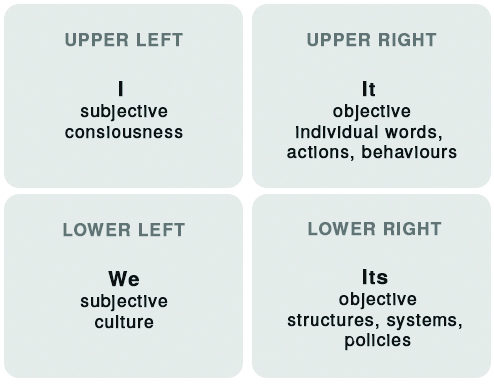
\includegraphics[width=0.65\textwidth]{./Images/laske-integral}
\caption[Experienced reality of work]{The experienced reality of work, the mental space that each person's work occurs in\cite{laske-vol2}.}
\label{fig:integral-organisation}
%\end{wrapfigure}
\end{SCfigure}


20 years ago, early in my career with P\&G,\index{Procter and Gamble} I (Graham) came across the phrase \emph{Culture eats strategy for breakfast}. I learnt to see culture as the final determinant of turning energy into results, after purpose, strategy, structure, processes, people etc. have done their bit. The longer I work in organisations, the more I realise just how true that is, and more importantly, the implications for how to create organisations that thrive in the face of adaptive challenges, and to build a better world.


If a proposed change to the structure, strategy, etc. of an organisation is contrary to the meaning\hyp{}making stories (culture) which shape and create the reality experienced by all stakeholders, the change is almost certain to fail, and may even break the organisation, no matter how much good the change might bring.


In just the same way that you will usually fail to change a behaviour that your meaning\hyp{}making stories tell you is wrong, or even harmful, regardless of how logical the new behaviour is.


The diagramme in Figure~\ref{fig:integral-organisation} illustrates how it all ties together. This is the standard diagramme from Ken Wilber's\index{Wilber, Ken} integral model. This captures quite clearly why culture is the biggest lever, and why I regard an organisation as a living being.


\begin{description}
\item[Upper Right (UR): Visible Individual] All the output your business delivers lies in the upper right quadrant. This is the quadrant where all visible activities of every single individual and the organisation lie. All output is ultimately individuals turning their energy into output through acting, and what they do is driven by the other three quadrants. Every action is compliant with the forces of the lower right, lower left, or upper left quadrants.


\item[Lower Right (LR): Visible Collective] Lower right is the other visible quadrant. This is where everything tangible related to your organisation lies. Your visible organisational structure lies here, your organisational chart as it stands on paper lies here, your explicit rules and policies lie here. In any of the Ocracies the circle structure, and the explicitly stated role domains, accountabilities, and drivers lie here. Your explicitly declared company strategy lies here. This quadrant drives compliance through the use of explicit rewards and punishments to impose adherence to prescribed structures, processes, and relationships. The Management Accountability Hierarchy (MAH)\index{Management Accountability Hierarchy} describes the organisation when you look at it through a lens showing this quadrant.


\item[Upper Left (UL): Hidden Individual] Upper left is where individuals’ unique meaning\hyp{}making stories, values, biases, personal energy economy lies; along with everything else that is hidden and nebulous. If everything you do in your personal upper right is fully in accord with your upper left, all of your activities are compliant with your meaning\hyp{}making essence as a human being. Your conscience, sense of guilt and shame drive one side of your compliance; your sense of joy, mastery etc. drive the other side.


\item[Lower Left (LL): Hidden Collective] Lower left is where the organisation's culture lies, your collective meaning\hyp{}making stories, as well as the nebulous, invisible organisation structure and hierarchy that enables you and your colleagues to deliver results despite visible organisation structures, hierarchy, rules and regulations that block you from delivering results. The actual, implicit company strategy lies here. Upper right actions are often compliant with lower left. If you look at it through a lens that highlights this quadrant, you see an organisation to be a Human Capability Hierarchy (HCH).\index{Human Capability Hierarchy}
\end{description}


\emph{Culture eats strategy for breakfast} summarises\index{culture} clearly that the driving forces are far stronger in the hidden, left than the visible lower right quadrants. The primary driver of what you and your colleagues do at work is everything that you cannot see, is nebulous, and where the only data that you have  lies in your nebulous feelings. 


The biggest lever you have to improve your business output is a nebulous, invisible one.


These quadrants capture perfectly how inherently, irreducibly uncertain and nebulous any organisation is. Each organisation is at once inseparably both lower right and lower left, and each quadrant apart has validity. Looking at this through the lens of a quantum physicist, they look analogous to the complementary pairs of a photon. 


Some approaches look at an organisation as just the lower right MAH, and everything lower left is a consequence of the lower right. In other words, once you get the visible organisation design, hierarchy, roles and circles, policies, and statutes of incorporation right, as an MAH, the organisational culture will fall into place.


Other approaches say that once you get the organisation's culture to be healthy, the most effective and efficient organisational design, an HCH, will emerge.


Looking at this as a quantum physicist, I can only conclude that an organisation is both HCH and MAH; and more, in an inherently nebulous, unknowable fashion. 


Perhaps we never can describe clearly what an organisation is, but only what we can say about what it is; just as physics\index{physics} is the study of what we can say about what is, not the study of what is.


Similarly, the best we can say about an organisation is that it is somehow both lower left and lower right, in a nebulous, contradictory way that we will never be able to pin down precisely in all dimensions and details. Just like an electron.


If you choose to look at your organisation through a lens that gives you maximum knowledge of the lower right, you will have the least or even no knowledge of the lower left. And vice versa. They are complementary pairs.\index{complementary pairs}


The best you can do with such complementary quantum pairs in physics is defined by Heisenberg’s \index{Heisenberg, Walter} uncertainty principle.\index{uncertainty!principle} There is a similar analogy to the uncertainty principle at work here too. Just as the uncertainty in quantum physics is an inherent uncertainty in nature, so too is this an inherent uncertainty in the organisation. The organisation itself does not and cannot consciously know everything that is happening in the lower left quadrant. As soon as you even look at the lower left quadrant, it will change, and what the lower right quadrant is actually driving in behavioural compliance of individuals will immediately begin changing away from what it was.


Looking at organisations as living meaning\hyp{}making beings integrates lower left and lower right, just as looking at yourself as a living meaning\hyp{}making being integrates upper left and upper right. 


If you want better results, you and all your colleagues need to become more effective and efficient at converting your human energy into results. This means you need to work with the internal reality of the workplace that each of you constructs from the hidden individual and collective meaning\hyp{}making stories.


Lower left compliance in most workplaces is a more powerful driver of your internal workplace experience and your actual productivity than lower right compliance (culture eats strategy). Perhaps the only workplace where lower right compliance is a more powerful driver is in slavery, and similar workplaces.


Look at the difference between the experienced work reality of each individual, i.e., their inner workplace, and the outer workplace that lies in the upper and lower right quadrants; it should become immediately clear to you how inherently nebulous designing the optimal organisation is. You simply cannot measure everything important, and not everything you can measure is important, as Einstein\index{Einstein, Albert} would have put it. Even more, once you have measured it, or even talked about it with a consultant, it has been changed by the process of measuring. 


This also makes clear that improving results has relatively little to do with skills and competencies and far more to do with the developmental nature of each individual, covered in Chapters~\ref{chapter:who-am-i-base} to~\ref{chapter:who-am-i-one}. All the work that you and your colleagues do comes from the self-constructed reality of each of your inner workplaces.


Another consequence of this is that there is no empirical justification for segmenting the members of your business into distinct categories like employees, managers, customers, investors, suppliers, family and community etc. The organisation as a whole is both lower left HCH and upper right MAH like any other living being, a constantly nebulous, undefinable flux shaped by the interactions of all stakeholders with each other across all four quadrants. 


To do justice to what an organisation actually is, especially in today's world where we need Adaptive Organisations with their full power and developmental capacity, we need to re-examine all of our current stories of what a workplace is, from the legal stakeholder level structures, the visible and invisible MAH and HCH, and each individual's developmental essence as a living, meaning\hyp{}making being.


As you structure your organisation, by looking at it as a living, meaning\hyp{}making being, a scaled-up version of yourself, it ought to be clear that any mismatch between an organisation's structure or process and the organisation's stories will be expensive, at best, and at worst lead to collapse. \index{Integral Organisation|)}






\section{Four layers, three dimensions in an organisation}
\label{section:adaptive-organisations}


In many ways the Adaptive Organisation and the Living Organisation are synonyms. I refer to a living organisation when I want to emphasise the nebulous, impossible to pin down essence of a living, meaning\hyp{}making being. I refer to an Adaptive Organisation\index{Adaptive Organisation} when I want to highlight the driver for that organisation to exist lies in its capacity to rise to adaptive challenges that require changing the collective and individual meaning\hyp{}making stories creating the organisation’s reality and identity.


If you look at an adaptive living organisation only through the lens of complex adaptive systems, you are blind to these meaning\hyp{}making stories as the most powerful things that shape the organisation's reality. 


Since most of these stories are hidden, you can only get at them if you use the living organisation lens, pay very careful attention, and do a lot of subtle detective work to deduce them without causing major disturbances in the process. 




\subsection{Four layers}


An organisation has four layers, \index{organisation!four layers|(} the lowest four layers listed in Section~\ref{section:harnessing-conflict-intro}.
\begin{description}
\item[4 Inter-organisational] How stakeholders\index{stakeholders} at the big picture level are dealt with. First and foremost here is the choice of legal incorporation, and then the processes used during general meetings and any other forum where stakeholders and the company interact with each other. The FairShares Commons incorporation is the best I currently know of for almost all kinds of entities, except perhaps a pure trust, or a wholly owned subsidiary of a FairShares Commons.\index{FairShares Commons} 
\item[3 Inner-organisational] How work gets done, and tasks deliver results. This spans how tasks are organised, the organisation design and power hierarchy, the visible decision-making processes, in fact, everything that is sometimes narrowly defined to be “the organisation”. Sociocracy, Holacracy, \index{Sociocracy} and other forms of dynamic organisation design or governance do this well. \index{Holacracy} 
\item[2 Inter-personal] How individual human beings interact with each other, their relationships, and how they bond into teams to pool their collective energy and activity into delivering bigger results than any one of them could ever have done alone. The Evolutesix Adaptive Way \index{Adaptive Way} for teams increases the organisation’s effectiveness really well.
\item[1 Inner-personal] How individuals and groups of people interact, how they develop themselves, and how they are in relationship to each other. The Adaptive Way for individuals also does this really well, covered in Part~\ref{part:you}.
\end{description}




Looking at these four layers through the living organisation lens, you can see that each layer contributes in different ways to the three elements of Equation~\ref{eq:living-organisation}. Each layer is essential for the entire organisation to be fully alive. If any layer is constrained in its freedom to live, the organisation as a whole is constrained in its capacity to thrive and deliver the output expected of it.


Each of these four layers and the interfaces between them must be optimised for whatever challenges we are facing. Most of our past experience is in optimising them to face and thrive in a world of technical challenges, experience holding us back now, when building an adaptive living organisation that can thrive in a world of adaptive challenges requires a very different optimisation. An adaptive living organisation, with all layers at full strength, is the ultimate learning organisation\cite{senge-fifth}.


Regardless of whether your organisation is only optimised for technical challenges or also for adaptive challenges, these four layers can only change within the constraints imposed by your organisation’s meaning\hyp{}making stories. 


This is especially relevant if you are leading an organisation that’s optimised to overcome technical challenges, and have decided to transform all four layers to become an Adaptive Organisation \index{Adaptive Organisation} with the potential to thrive in the adaptive challenges ahead of you. You are unlikely to be making this journey unless you work simultaneously on making the meaning\hyp{}making stories of the living organisation lens visible, growing them to become bigger and more adaptive, and only changing any of the four layers within the boundaries of your stories.


I have seen many well-intentioned leaders recognise the imperative for their organisation to become an adaptive one and dive headfirst into the deep end of changing only one of these four layers, immediately rolling out the flavour-of-the-month approach from the top down. All too often these attempts crash and burn, because the meaning\hyp{}making stories of the individuals and the organisation as a whole do not support this approach, or they support the “why and what”, but not the “how” of the path of change\footnote{Organisations are clearly not ergodic. \index{ergodicity} Where you are now depends crucially on the path you took from where you were, and very little on the characteristics of where you were and where you are.}. 


\begin{longstoryblock}
One example that comes to mind is typical of many. The organisation was a small consultancy, formed by a group of people in their early 30s who had a very clear vision to create a company that was different to any traditional consultancy. In many ways they were at the cutting edge of visionary experimentation towards Adaptive Organisations.


The personal energy economics (described in section~\ref{section:PEE}) of the founders was superbly complementary. During the very first meeting I had with them, I pointed out how they could form a superhuman if they figured out how to put Peter Drucker's dictum fully into practice, by organising and collaborating in such a way that their strengths were made fully productive and their weaknesses irrelevant. They could have been the model case study of an adaptive living organisation.


Unfortunately, their living organisation had other deeply hidden and more powerful meaning\hyp{}making stories in it. These were stories about what it meant to succeed and fail, stories about vulnerability, safety, and security. Stories harming their aspiration to flourish by standing together in their common oneness in ways that supported each individual's uniqueness. 


The organisation imploded less than a year after they began seriously implementing Holacracy, leaving a shadow of its full potential still living. The living organisation’s dominant hidden stories created the reality that everybody experienced, and it was not one that people were willing to live in.
\end{longstoryblock}


I've experienced this time and time again in organisations that I have worked with, and people who I've spoken to. 


On the other hand, the success stories I've heard fall into two categories. Either the meaning\hyp{}making story of the living organisation was big enough and ready enough for the change destination and path, so it welcomed the change and the change worked. Or, the change or the path did not fit into the organisation's meaning\hyp{}making story, and the change agents recognised this soon enough to dial back the change to something that did fit within the living organisation's meaning\hyp{}making story. And then step-by-step grow the story just before taking the next step along the path to organisational change.\index{organisation!four layers|)} 
\subsection{How adaptive is your organisation?}
If your organisation is going to thrive because it can rise to the adaptive challenges ahead of it, you need to know how adaptive it is. The rest of this chapter will enable you to understand just this. 


Darwin\index{Darwin, Charles}  recognised that whenever any life form no longer fits the context and need, or driver, of its niche in the ecosystem, the conflict created provides both the direction and the motivation for change. In the language of Darwin's time, this was the meaning of survival of the fittest. It had nothing to do with how many currently perceive his words, that the stronger and more aggressive you are, the better you will survive. Darwin was quite clear that if the best fit to a niche in the ecosystem lay in altruistic collaboration, the species most able to collaborate altruistically would thrive.


The conflict in and between these four layers contains valuable data on where you and your organisation are poor fits to the driver of your niche in society and its economy. The bigger your adaptive capacity, the more likely you are to be able to mine and refine this data to evolve at least as fast as your niche is moving.


There is conflict\index{conflict} within each layer. (And, more complex,  between layers.) 
\begin{enumerate}
\item The stakeholder arena, where the conflict between the different stakeholder interests and meaning\hyp{}making stories.
\item The task arena, where human energy gets transformed into business results.
\item The interpersonal arena, between two or more people in an organisation. This is where the organisation’s culture is created and is the primary shaper of the reality that the organisation as a whole experiences.
\item The personal arena, the conflict inside you between the different facets of who you are.
\end{enumerate}


All four conflict arenas are at the heart of the challenges humanity is facing. Until we figure out how to do what nature has done so well from the beginning of life on the planet, namely mine and refine conflict as the driver for how to evolve to face the adaptive challenges, we will fail to sufficiently address our climate crisis.


I am optimistic, because we already have clarity on what to do in each of these four conflict arenas. We already have more than enough success stories of individuals and organisations who have used one or more pillars to increase their organisation’s adaptive capacity. An excellent example of someone practising this, harnessing conflict individually and in his organisation, is Ray Dalio\cite{dalio-principles}, \index{Dalio, Ray} the founder and CEO of Bridgewater, one of the world's largest hedge funds.\index{Bridgewater} 


\subsection{Three dimensions}
The capacity needed for a living organisation to be healthy in all four layers requires the right structures and processes in each of the three dimensions of Figure~\ref{figure:three-axes}. The following three chapters deal with each dimension in turn.


\begin{figure}
\begin{center}
\includegraphics[width=0.95\textwidth]
{./Images/0Zoom-AO-Axes-White}
\end{center}
\caption[The three dimensions of an organisation]{The three dimensions of an organisation. Most of the possible points your organisation could sit at are at best only stable for a short period, at worst extremely fragile.}
\label{figure:three-axes}
\end{figure}


The key message to keep in mind as you read each of those chapters: to create an Adaptive Organisation, \index{Adaptive Organisation} or Teal, \index{Teal} or whatever name you prefer, you need to aim for Level 5 on each axis. 


Take psychological safety, for example. Some organisations attempt to deliver that by working on the culture\textemdash the human axis. Yes, that’s where psychological safety lies; but you cannot create long-lasting antifragile psychological safety \index{psychological safety} if your roles and tasks dimension is less than Level~2 Self-Managing; nor if your incorporation is anything less than a Level~2 worker coop. And even having both of these on level 2 is barely adequate for psychological safety. 


If you really want antifragile, long-lasting psychological safety\textemdash at the level you need to maximise the Job~1 energy\textemdash you need to strive for Level~5 incorporation (Free company / FairShares Commons) and at least a self-directing Level~4 in roles and tasks. 


This is why so many efforts to create humane, self-managing, or deliberately developmental organisations fail. They act in only one dimension, maybe two, but miss the third. Most commonly the incorporation is the missing dimension. 


Move forwards on all three; moving far on just one or two is recklessly fragile.  
 
\section{The vision and purpose problem}
Losing connection with the source (Section~\ref{section:source}), the driver to becoming a living being, is the reason why many organisations have run into trouble with their purpose and / or vision statements in today's world. 


Very few businesses have a vision statement that is of any use in creating an organisation with long-term viability. Most vision statements are visionless. They say something like \emph{we want to be the best in the world.} There's nothing wrong with aiming to excel, but vision statements are dysfunctional in facing the global adaptive challenges we all face today, because they create a sharp divide between everybody inside the organisation / the winners, and everybody outside the organisation / the losers. 


Such vision statements \index{vision statement} exclude most possibilities for collaboration, and meeting the human needs of bonding, altruism, etc., listed in Table~\ref{table:needs-top}. Any vision statement that is not inviting and energising to every single stakeholder in the business: staff, customers, suppliers, their families and descendants, the communities and nations they live in; is at best unhelpful and at worst harmful. By excluding sharply, such a vision statement sows the seeds of business collapse from day one. It's not for nothing that the oldest organisations in the world are centred around all stakeholders.


The other kind of vision statement articulates clearly some ideal better world. This vision statement is far more likely to lead to long-term viability, and to invite contributions from a wide pool of stakeholders who all sign up to that vision of a better world. The problem with such a vision statement is that it easily becomes concretised. The vision statement takes on an independent life of its own and continues to drive, unquestioningly, the activities of the business and everybody in it, long after its sell-by date.


Purpose statements are a significant improvement on many vision statements that are out there. For example, during my time (Graham) at P\&G’s stated purpose was \emph{improving the lives of the world's consumers}. That clarity of purpose was one of the initial attractions for me of working there. A consequence of that clarity of purpose was the very clear recognition that the consumer was boss. If the consumer data pointed at one option, and an individual in senior management demanded that the team choose a different option, we seldom needed much discussion, once we had solid data on the consumer preference. 


However, the longer I worked in P\&G, \index{Procter and Gamble} the more I began to realise just how the choices we were actually making were also being shaped by a dominant hidden story. This dominant hidden story was meeting the quarterly investor expectations, and delivering total shareholder return (TSR). \index{Total Shareholder Return} It became clearer that this quarterly TSR focus was sometimes leading us to make choices that were not truly in the interests of the world's consumers today, next year, and seldom good for future generations.


That purpose statement was very close to being a driver statement; it was implicitly anchored in the external world. But because it lacked a clear articulation of the external context and need, it was nearly impossible to recognise when the dominant TSR story was, so shaping the reality we experienced that it was no longer anchored in meeting the external need; and no longer aligned with our purpose.


The current push towards for-purpose enterprises is a huge step forwards vs. the traditional approach of not defining a purpose in the statutes, leaving it to be deemed as TSR. We can do even better: the evolutionary enterprise with the explicit driver. This addresses an Achilles heel of for-purpose and perpetual purpose companies: what happens to a perpetual purpose company when something big changes in the context and need that that purpose exists to meet, if it loses connection with that driver?






\section{First drivers, then objectives and purpose}
\label{section:driver}
The rise of the for-purpose organisation\index{organisation!for-purpose}  is one of the most important developments over the past decade. In most countries, company law makes clear that an organisation exists to fulfil its purpose, and the executives’ fiduciary duty is to maximise the organisation’s capacity to fulfil its purpose.


However, few founders have their organisation’s purpose clearly stated in the legal documents of incorporation. And so, when things have ended up in court, lawyers and judges have needed to come up with a definition of what the implicit purpose then is. Given the nature of the neoclassical economics\index{economics!neoclassical}  meaning\hyp{}making story, the default was that the organisation’s purpose was to maximise total shareholder return.


More founders are now perfectly clear that you cannot leave defining the organisation’s purpose in the hands of lawyers after things have gone wrong. You must express it very clearly before you even incorporate it. 


When Dee Hock\cite{hock-one} \index{Hock, Dee} was creating Visa \index{Visa Corporation} during the 1960s to bond all of the world's players in the emerging credit card industry, he was able to do that because he had a very clear idea of the context and need, making it easy to define a purpose that aligned all stakeholders.


Hock later coined the term “chaordic” \index{chaordic}  to describe the process he used to find the purpose of Visa and create the organisation. He had realised that in nature, the best evolutionary leaps emerge right on the boundary between order and chaos. He recognised clearly that evolution anchors itself in the immediate context and whatever is needed within that context. I read his book, \emph{One from Many: Visa and the Rise of Chaordic organisation}\cite{hock-one} every few years, and every time I read it I uncover deeper brilliance in his insights.


The starting point of Dee Hock's Chaordic Organisation I call \emph{the driver}, to my knowledge first named as such in Sociocracy~3.0\cite{priest-s3-web}. The driver comes before any purpose. The driver is the combination of the current environment and the need calling to be met. The purpose is then trivial: to always meet the need, within the constraints and possibilities of the current environment. 


Anchoring yourself and your organisation in a driver, rather than a purpose, keeps the organisation at the emergent edge of evolution. The driver statement is a tool enabling an organisation work with its evolutionary purpose (see Frederic Laloux's book \index{Laloux, Frederic} \emph{Reinventing organizations}\cite{laloux-RO}). \index{Reinventing Organizations} 


Explicitly stating the driver in the statutes addresses a weakness in almost all purpose statements I have seen: the loss of contact with the changes to the driver the original external founders' first concretised into a purpose. In the worst case this loss of contact means a business putting all its resources and energy into continuing to fulfil a purpose long after the driver has ceased to exist, the purpose irrelevant, and so becoming a zombie company \index{company!zombie} eating investors and staff.


We are strongly for going beyond a for-purpose company to an evolutionary enterprise, where the company’s strategic objectives and legally anchored objects are stated in terms of the evolutionary driver. 




\section{Changing a living organisation}
\label{section:change-living-organisation}
\begin{quote}
One is led to a new notion of unbroken wholeness which denies the classical idea of analysability of the world into separately and independently existing parts. We have reversed the usual classical notion that the independent elementary parts of the world are the fundamental reality, and the various systems are merely particular contingent forms and arrangements of these parts. Rather, we say that the inseparable quantum interconnectedness of the whole universe is the fundamental reality, and the relatively independently behaving parts are merely particular on contingent forms within this whole.\\
\raggedleft\textemdash David Bohm, Physicist
\end{quote} \index{Bohm, David} 


Given everything that you have read so far, you might be asking yourself, 


\begin{quote} 
so how on earth do you even begin changing an organisation?
\end{quote}


As Jack and I were writing this book, the above quote from David Bohm was very present in what we were doing. David Bohm later left physics and pioneered a dialogue process that enabled people to experience their common interconnected oneness as primary. Not the only physicist to move into dialogue processes! 


Do you see an organisation as primarily many individual human beings that just happen to be in and serving it, or do you see an organisation as primarily the web of interconnections and activity, in which the people who are there just happen to occupy key points in the interconnected oneness? Do you see an organisation deriving its nature because of the people, or the people deriving their nature because of the organisation?\index{organisation} 


The reality you create and experience in your organisation, especially in any attempt to change it, will depend on which meaning\hyp{}making stories you use. 


It has become clearer over the past few decades that it's often far more accurate to say that the reality of an organisation is the indeterminate, spread-out continuum of interconnections; the processes that move and change things from A to B; the relatedness of different aspects; the relationship between the people; the interactivity between people and between roles; and how all of that can be and is in constant transformation.


This means that when anything needs changing, the biggest levers to create that change, and therefore the place to start, lie everywhere. The most powerful though lie in the collective and individual meaning\hyp{}making stories, and growing each individual’s \index{Size of Person} Size of Person. 


Compare that to the change process that you typically find today in organisations, primarily centred on the people. Often starting by replacing the CEO.


The corollary of this is the belief that we need to pay individual CEOs extremely high remuneration packages.


If the whole organisation’s interconnectedness is the fundamental reality, and the relatively independently behaving people are merely particular forms within this whole (multiple thought forms from Chapter~\ref{chapter:who-am-i-sense} are used here), then it doesn't really matter which CEO is in place, so long as they have the right developmental Size of Person, skill set, and motivation to be a strong connector in the CEO role constituted by the pre-existing relatedness created by the organisation. The CEO themself is just background. The foreground is everything else, including the entire organisation as a living being. 


The behaviour of individuals derives its nature from the whole, as an expression of the whole. Paradoxically, this actually makes it easier to work with behaviour in organisations when changes are needed. 


To improve results, especially for the long term, shift from looking at individuals to looking at the whole as a living being, and as an inseparably interconnected nebulous intangible ecosystem. 


First of all, because it eliminates the entire paradigms of individual blame and shame. This immediately shifts, into productive effort, all the time and energy people put into preventing themselves getting into situations where they might be blamed for something, protecting their vulnerabilities, looking good at work, impressing the boss, etc. 


Secondly, instead of a large number of managers and HR professionals trying to get to grips with every single individual in the organisation, and how to change each individual in the organisation, the focus becomes setting up an organisational condition that naturally has the behaviour you need because that behaviour is simply the most probable behaviour. The behaviour equivalent to a particle in physics moving in a straight line because no force is acting on it.


Just as you read in Chapter~\ref{section:optimised-self} about having optimised who you are today as the best possible living being you could be to overcome the challenges of your past, so too your organisation as it is today is optimised for its past challenges. Not for its current challenges, let alone its future challenges.


Unless your organisation is firmly anchored in the external challenges of today, you run a high risk of disappearing in the near future. If you want it to thrive long-term, you cannot do better today than anchor yourself in the best possible understanding of the challenges that the future will bring.


This means anchoring your organisation in a relevant driver statement: the external context and need your organisation chooses to meet. Regularly check for changes in the external context or need, and immediately update the driver statement to match. Put an expiry date (or expiration in the US) into your driver statements, to trigger that checking process on regular intervals. Without an expiry date, it's all too easy for you to lose sight of the original driver, concretise the purpose that comes out of that driver, and then continue to act on the purpose, even though it's no longer as relevant to your success (thought form P6).


\begin{SCfigure}
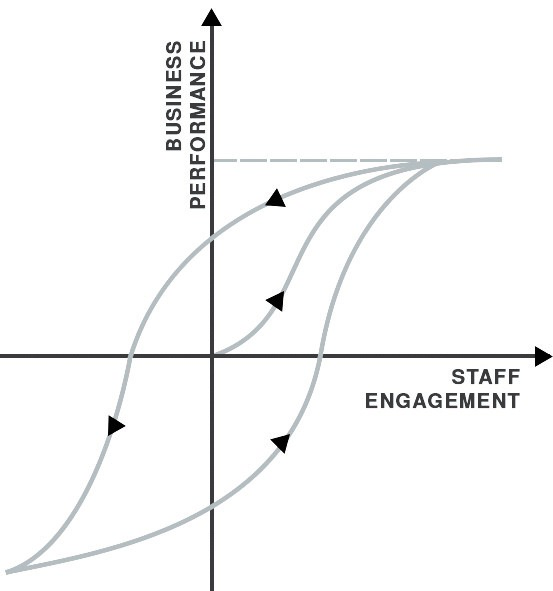
\includegraphics[width=0.49\textwidth]{./Images/hysteresis}
\caption[Hysteresis. Business performance vs. staff engagement]{Hysteresis. As  staff engagement, motivation and Job 2 energy loss changes, this is the path business performance moves along over time: from funding the startup to maturity, then the response to a threatening change, and the recovery. Or collapse, more likely, as few businesses ever recover from the leftmost point. }\label{fig:hysteresis}
\end{SCfigure}


Changing existing organisations to this way of working is, in many cases, a bigger challenge than starting a new organisation. Changing requires you to first get your company back to zero before you can build it up to a new place. Once your organisation\index{organisation}  has been running for any significant length of time, you have investors on board, the story that defines who your company is and how people interact with each other has embedded itself and attracts people who reinforce that story. 


Figure~\ref{fig:hysteresis} depicts what often makes surviving a change impossible, and how many things behave when you try to change them. You can see here the path that many organisations will go on. The organisation begins at zero and climbs in an S-curve to wherever it is now. The vertical axis represents profitable business output. The x-axis represents staff engagement, and how much energy they are putting into their work.


You can see in the upper curve, with the arrow going back, that initially employee engagement and effort drops significantly before there is any measurable impact on business performance. By the time the curve has dropped far enough for senior management to have clear data that something is seriously wrong, average engagement has gone through zero and continues to plummet.


By the time the consultants have been brought in, analyses have been made, and a plan of action is in place, staff engagement is even lower. If it is a good plan, staff engagement begins to rise. But, critically, it rises along the lower curve. It does not go back along the upper curve. This means that while staff engagement begins to move towards the positive, it needs significant growth before there is any business-relevant increase in output.


In many businesses the wealth of social capital (patience, trust in senior management and the investors, etc.) and financial capital has already been so far depleted before action is taken to get productivity above the line, and back into sustainable profit, before the company collapses. 


This is why it is very hard, after you have cast the first foundation stone, for any of the approaches described in these chapters to fix the problems. Start when you found the company, not when you finally realise you are in trouble.


It is also important to guard against any of your cognitive biases, leading you to believe what is false\cite{wiseman-paranormality}. You may only have one, at most two attempts; do not waste them. Protecting yourself against sleight of hand, illusion, and the seductive appeal of false certainty\cite{kuhn-magic} is an ongoing application of thought form P6; and gets harder the more your business drivers are Cynefin complex or chaotic.


A book that shaped my thinking on how self-governing could deliver extraordinary business results, and that guided me (Graham) when I took over the section in Beijing P\&G, \index{Procter and Gamble} is Tracey Kidder's, \emph{The Soul of a New Machine}\cite{kidder-soul}, \index{Kidder, Tracey} the story of how a team of computer geeks in a skunkworks program created the 32-bit minicomputer that could have built the bridge for Data General to become a successful company in today's PC era.


I strongly recommend you read this book if you are working within an existing company, and want to build a self-managing team, especially if you have the hope that this will be the positive disruptor that turns your whole organisation into a self-managing team. The book tells the story of how the team leader, Tom West, created a story within the team where they were or on a hero's journey to save the company from the recently released VAX of Digital Equipment Corporation. The book also tells the story of the brutal political battles he needed to fight to make sure that the team was protected from the rest of Data General. \index{Data General} 


The team’s success in delivering what nobody thought could be delivered, their beating (time, resource usage, and final profitability) the official team developing what management had intended would be the VAX beater, lay in Tom West running the team according to some of the principles we have just discussed. 


I believe that a key reason why Data General was unable to use this success as its bridge into being one of today's most successful companies in the computer world lies in its management not recognising the power of this way of working. And I believe the reason for that lies in it having a traditional incorporation. Read the update, published 20 years after the team delivered its computer, in Wired\cite{ratliff-wired-soul}.


Just one story of organisations failing because they have been optimised to rise to technical challenges. We will never be able to rise to the global adaptive challenges we are all facing today if we continue trying to do the same as we've done before, only harder. Throwing more money at our current adaptive challenges is only going to make them worse, unless we work with our businesses as adaptive living beings.